
\subsubsection{Generator\label{sec:Generator}}

The generator is the module responsible for generating Java classes
and interfaces for a specific instance of the meta model.

The generator generates the following:
\begin{itemize}
\item Interfaces and classes for each Value Domain defined in the environment
and the data models.
\item The environment class that contains the instance factories for each
data model in the environment.
\item An instance factory for each data model in the environment, that controls
the individual instances of the data model.
\end{itemize}
For each data model in the environment, the following is generated:
\begin{itemize}
\item The set of interfaces that makes up the internal API, used by the
actions and views to manipulate and view the state of the data model
instance.
\item The set of classes that implements the internal API and binds it to
the runtime interface.
\item The stub classes where the user implements the actions and view. There
is one stub class for each action and view.
\item The external interface for the data model.
\item The implementation of the external interface, that binds the methods
of the interface to the stub classes and execute them through the
runtime interface.
\end{itemize}

\subparagraph{}


\paragraph{\label{sub:Creation-of-values}Value Domains}

The value domains are the type system and infrastructure in EDMA that
binds everything together and ensures that every part of a project
speaks the same language. Each value domain represents a unique type
of data with a well defined structure.

The generator generates two classes for each defined value domain:
An abstract class that serves as an interface to values from the value
domain and an implementation class that implements the abstract methods
in the interface. The reason for using an abstract class instead of
a Java interface is that Java does not support static methods in interfaces
and there are several static methods used to create new values:
\begin{itemize}
\item create - this method creates a new value from scratch 
\item fromString - this method creates a new value from the string representation
of the value.
\item fromStream - this method reads a value from a stream.
\item fromStreamNoValidate - this method reads a value from a stream without
validating it. It should only be used when reading from a trusted
source. For large complex values with many constraints the validate
process could be slow, that is the reason for having this method.
\item fromTerminal - this method uses a terminal to instruct a user to create
a new value.
\end{itemize}
And some abstract methods:
\begin{itemize}
\item toString - returns the string representation of the value.
\item toStream - writes the value to a stream.
\end{itemize}
All value domain classes also have sensible implementations of the
comparable interface, the hashCode and equals methods.

The create method for struct type value domains uses a modified version
of the builder pattern to create new values. The builder pattern uses
what is known as a fluid interface\cite{fowler2008}, where methods
are chained together. This results in more readable code, where each
field has a set-method named after it. In EDMA we have taken the builder
pattern one step further, so each field has its own interface, with
a set-method named after the field. Each set-method then returns the
builder-interface for the next field except the last one, which returns
the created object or value. By doing it this way, we get a fixed
order of the attributes and we make sure that it is not possible to
miss out on any of them. It would be a bit cumbersome to program this
by hand, but with auto-generated code it is no problem. As an example,
lets see how we would create a new date from the date value domain:

\begin{lstlisting}[language=java,frame=none]
Date myDate = Date.create().year(1973).month(6).day(7);
\end{lstlisting}The static method \texttt{Date.create()} returns an interface that
only has a method for setting the year. That method returns an interface
with a method to set the month, which in turn returns an interface
to set the day. The interface for setting the day finally returns
the completed data value. If we put the attributes in a wrong order
or if we missed out any of them, then the Java compiler would complain
immediately. If the user uses a modern IDE e.g. eclipse, it gets very
easy since the automatic code-completion will pop up with the name
of the next field after each dot. This type of chained interfaces
are used in EDMA both when creating values from value domains and
when creating entities from kinds.


\paragraph{Data Models}

For each data model in the environment, several interfaces and classes
are created:
\begin{itemize}
\item Data model factory interface. This interface provides methods to create
new instances of the data model and to get access to existing instances
of the data model. Each instance is identified by a name.
\item Data model instance interface. This interface is used to start and
stop the instance and to get the external interface of the instance.
The methods of the external interface can only be called when the
instance is running. Otherwise an exception is thrown.
\item Data model external interface. This is the external interface of the
data model that clients can use to execute the actions and views on
the data model.
\item Internal view interface. This is the interface that \emph{views} use
internally to navigate and extract information from the data model.
\item Internal update interface. This interface extends the internal view
interface and adds functionality to make changes to the data model.
This is the interface that \emph{actions} use internally.
\end{itemize}
Besides these interfaces there are also generated classes that bind
these data model specific interfaces to the general runtime interface.


\paragraph{Kinds}

For each kind in the data model we create a number of interfaces that
can be used internally in the implementation of the views and actions.
These interfaces are:
\begin{itemize}
\item The entity view interface. This interface provides methods to read
the attributes of an entity of this kind. It will also get the methods
that are used to navigate any relations that this kind is part of.
\item The entity update interface. This interface extends the view interface
and adds methods to update the mutable attributes. This interface
will also get methods to create and delete connections with other
entities through the relations that this kind is part of.
\item The set interface. This interface is used to navigate sets of entities
of this kind. It implements the iterable interface and has methods
to create new sets by unions, intersections and subtractions with
other sets of the same kind. It also gets methods to navigate relations
that this kind is part of.
\item The filter interface. This is a simple interface that can be used
to create specialized filters that can be used on sets of entities
of this kind.
\item The kind interface. This interface has methods to get access to all
entities of this kind or a specific entity either by ID or by any
unique index on the kind. It also has methods to get access to specific
sets of entities based on the indexes declared on this kind.
\end{itemize}
For each kind in the data model, the internal view interface for the
data model gets a method to access the kind interface and the internal
update interface gets methods to create new entities and delete entities
of this kind and a method to upgrade a view interface for an entity
of this kind to an update interface. For singletons we only have the
entity view and entity update interface.

The way we update entities is a little special because of the unique
index. Normally we would just make a set method for each mutable attribute
and then these could be used to update entities one attribute at the
time, but this could give problems if there are unique indexes that
span more than one attribute. As an example, lets say we have a person
kind with separate attributes for first name and last name and that
we have a unique index on (firstName, lastName). There exist a person
called ``John Andersen'' and another person called ``Thomas Andersen''.
Lets say we want to change the name of ``Thomas Andersen'' to ``John
Nielsen'', then we would get an UniqueException if we started by
changing his first name to ``John'', because now there would be
two people named ``John Andersen''. To solve this we have made it
possible to update several attributes at once. Instead of doing something
like this:\begin{lstlisting}[language=java,frame=l]
person.setFirstName("John");
person.setLastName("Nielsen");
\end{lstlisting}We instead do like this:\begin{lstlisting}[language=java,frame=l]
person.setFirstName("John").setLastName("Nielsen").save();
\end{lstlisting}Thus, we update both the first name and the last name at the same
time and we will only get an UniqueException if there is another person
named ``John Nielsen''. The \emph{save} method only declares that
it can throw a UniqueException if we actually update an attribute
that is part of a unique index. This is done by a little trick, where
we actually have two different interfaces for updating the attributes,
a \emph{plain} one where the \emph{save} method does \emph{not} throw
a UniqueException and a \emph{unique} one where the \emph{save} method
declares to throw the UniqueException. In the \emph{plain} interface
all set methods on attributes that are not part of a unique index
just return the \emph{plain} interface again, but the set methods
for those attributes that are involved in a unique index returns the
\emph{unique} interface instead. In the \emph{unique} interface all
set methods returns the \emph{unique} interface again. So this does
that as soon as we have ``touched'' an attribute that is part of
a unique index, then the \emph{save} method will declare that it can
throw the UniqueException.

Besides these interfaces there are also generated classes that binds
these data model specific interfaces to the general runtime interface.


\paragraph{Relations}

The relations in the data model add methods to the interfaces for
the kinds participating in the relation. The names of these methods
are dependent on the type of the relation, as well as names and roles
of the participating kinds. For example, having a relation \texttt{StudentEnrollment}
between \texttt{Course} and \texttt{Person} (having the role of \texttt{student})
results in four methods; two in the \texttt{CourseUpdate} interface
(\texttt{addStudent} and \texttt{removeStudent}), one in the \texttt{PersonViewer}
interface (\texttt{asStudentGetCourseSet}) and one in the \texttt{CourseViewer}
interface (\texttt{getStudentSet}). This is visualized in figure~\ref{fig:generatorRelations}.

\begin{figure}[h]
\rule{\textwidth}{.1mm}
\emph{EDMA file:}
\begin{lstlisting}[language=edma,frame=l]
Relation StudentEnrollment Course >-< Person:student
\end{lstlisting}
\emph{Generated Java:}
\begin{lstlisting}[language=java,frame=l]
public interface CourseUpdater {
	boolean addStudent(PersonViewer student);
	boolean removeStudent(PersonViewer student);
	. . .
}
public interface PersonViewer {
	CourseSet asStudentGetCourseSet();
	. . .
}
public interface CourseViewer {
	PersonSet getStudentSet();
	. . .
}
\end{lstlisting}
\rule{\textwidth}{.1mm}
\caption{Top: The relation as represented in the data definition language. Bottom: The generated code.}
\label{fig:generatorRelations}
\end{figure}Notice that the method in the course viewer interface is not named
\texttt{asCourseGetStudentSet}, but just \texttt{getStudentSet.} Methods
in the \texttt{PersonUpdate} interface for adding and removing courses
(as a student) could be generated as well; however, these would be
redundant with the \texttt{addStudent} and \texttt{removeStudent}
in the \texttt{CourseUpdater} interface. Therefore, the generator
only creates connection methods on the first kind in the relation
(the kind written to the left in the relation declaration).

In a one-to-many relation, a method returning a set of the other kind,
is created on the first kind, while a method returning a single entity
is created on the second kind. This is shown in figure~\ref{fig:generatorRelationsManyOne}.

\begin{figure}[h]
\rule{\textwidth}{0.1mm}
\emph{EDMA file:}
\begin{lstlisting}[language=edma,frame=l]
Relation TeacherAssignment Course >-- Person:teacher
\end{lstlisting}
\emph{Generated Java:}
\begin{lstlisting}[language=java,frame=l]
public interface PersonViewer {
	CourseSet asTeacherGetCourseSet();
	. . .
}
public interface CourseViewer {
	PersonViewer getTeacher();
	. . .
}
\end{lstlisting}
\rule{\textwidth}{0.1mm}
\caption{In a many-to-one relation, a method returning a set is generated on the one-part, while a method returning a single viewer is generated on the many-part.}
\label{fig:generatorRelationsManyOne}
\end{figure}In the \texttt{CourseUpdate} interface, a method is generated for
creating and deleting connections, as shown below.\begin{lstlisting}[language=java,frame=l]
PersonViewer setTeacher(PersonViewer teacher);
\end{lstlisting}This method returns the previous teacher, or \emph{null} if there
previously was no teacher assigned to the course. To remove the current
teacher without setting a new, this method can be called with \emph{null}
as argument.

\begin{figure}[h!]
\rule{\textwidth}{0.1mm}
\emph{EDMA file:}
\begin{lstlisting}[language=edma,frame=none]
Relation Marriage Person:spouse --- Person:spouse
\end{lstlisting}
\emph{Generated Java:}
\begin{lstlisting}[language=java,frame=none]
public interface PersonViewer {
	PersonViewer asSpouseGetSpouse();
	PersonViewer asSpouseSetSpouse(PersonViewer spouse);
	. . . 
}
\end{lstlisting}
\rule{\textwidth}{0.1mm}
\caption{In a one-to-one-self relation, a getter and setter method is generated as expected.}
\label{fig:generatorRelationsOneToOneSelf}
\end{figure}The one-to-one-self relation generates code as expected. Figure~\ref{fig:generatorRelationsOneToOneSelf}
shows a one-to-one-self relation, \texttt{Marriage}, relating two
persons, each with the role of \texttt{spouse}. In the resulting PersonViewer
interface, a method to get the spouse, as well one to set the spouse,
is generated.


\paragraph{Indexes}

There are three types of indexes in EDMA\emph{ (Unique}, \emph{Equal}
and \emph{Compare}) and each of these can be placed both on kinds
and on relations. When an index is placed on a kind, the methods related
to the index are added to the kind's interface. When an index is placed
on a relation, the methods are added to the entity viewer interface.
A Unique index does not only add extra methods to these interfaces,
it also adds a ``\texttt{throws UniqueException}'' declaration to
every method that might violate the unique constraint.

\begin{figure}[h]
\rule{\textwidth}{.1mm}
\emph{EMDA file:}
\begin{lstlisting}[language=EDMA, frame=none, tabsize=4]
Kind Person
{
	name : Name
	email : Email
	birthdate : Date
	Unique(email)
	Compare(birthdate)
}
\end{lstlisting}
\emph{Generated Java:}
\begin{lstlisting}[language=java, frame=none, tabsize=4]
public interface PersonKind {
	PersonViewer getFromID(PersonID id);
	PersonSet getAll();
	
	PersonViewer getFromEmail(Email email);
	PersonSet getWhereBirthdayEquals(Date date);
	PersonSet getWhereBirthdayLessThan(Date date);
	PersonSet getWhereBirthdayLessThanOrEqual(Date date);
	PersonSet getWhereBirthdayGreaterThan(Date date);
	PersonSet getWhereBirthdayGreaterThanOrEqual(Date date);
	PersonSet getWhereBirthdayInRange(
			Date minBirthday, 
			boolean minInclusive,
			Date maxBirthday,
			boolean maxInclusive);
}
\end{lstlisting}
\rule{\textwidth}{.1mm}
\caption{empty}
\label{fig:empty}
\end{figure}


\paragraph{Actions and Views}

Actions and views are the transactions in EDMA. For each Action or
View defined by a data model, a corresponding Java class is created
by the generator. These classes are the placeholders for the Java-code
that makes up the specific action or view. This is best illustrated
by an example: In the data model definition we define an action like
this:

\begin{lstlisting}[frame=l,breaklines=true]
Action createPerson
{
	Description:
		"Creates a new person"
	Input: 
		name : Name,
		email : Email,
		mobile : Mobile
	Output:
		id : PersonID
	ErrorCodes:
		1 - "Email already exists",
		2 - "Mobile already exists"
}
\end{lstlisting}

The generator will then generate the following java class:

\begin{lstlisting}[language=java,frame=l,breaklines=true]
...
public class CreatePersonUserImpl extends 
	Result implements CreatePersonResult
{
	private static final int OK = 0;
	private static final int EMAIL_ALREADY_EXISTS = 1;
	private static final int MOBILE_ALREADY_EXISTS = 2;
	private final Name in_name;
	private final Email in_email;
	private final Mobile in_mobile;
	private PersonID out_id;

	/**
	 * Constructor
	 * @param in_name    Input parameter 1
	 * @param in_email   Input parameter 2
	 * @param in_mobile  Input parameter 3
	 */
	public CreatePersonUserImpl(Name in_name, 
			Email in_email, 
			Mobile in_mobile)
	{
		this.in_name = in_name;
		this.in_email = in_email;
		this.in_mobile = in_mobile;
		out_id = null;
	}

	/**
	 * Execution of the action
	 * @param upd  Update interface
	 * @return     Return 0 to commit or one of the error codes to roll back
	 */
	public int execute(CourseRegUpdater upd)
	{
		// Implementation of createPerson
		// Return one of the following error codes:
		// OK
		// EMAIL_ALREADY_EXISTS
		// MOBILE_ALREADY_EXISTS
		
		// If an error needs extra explanation,
		// use: setErrorDescription("Extra info");
		
		// WARNING : Any code outside the following begin and end tags
		// will be lost when re-generation occurs.
		
		// EDMA_non-generated_code_begin
		
		//TODO : put your implementation here...
		throw new RuntimeException("This action has not been implemented yet!");
		
		// EDMA_non-generated_code_end
	}

	/**
	 * Returns the output id:PersonID
	 * @return  The output id:PersonID
	 */
	public PersonID getId()
	{
		if(errorCode() != 0) return null;
		return out_id;
	}
}

\end{lstlisting}

The user must now implement the business logic that makes up the action
using the interface provided as a parameter in the execute method.
The execute method must return one of the error-codes or 0 (OK) if
successful. The implementation could look like this:

\begin{lstlisting}[language=java,frame=l,breaklines=true]
...
	// EDMA_non-generated_code_begin
	if(upd.getPersonKind().getFromEmail(in_email) != null)
	{
		return EMAIL_ALREADY_EXISTS;
	}
	if(upd.getPersonKind().getFromMobile(in_mobile) != null)
	{
		return MOBILE_ALREADY_EXISTS;
	}
	
	PersonUpdater person = upd.newPerson()
		.name(in_name)
		.email(in_email)
		.mobile(in_mobile)
		.balance(NotNegInt.create(0));
	out_id = person.getID();
	return OK;
	// EDMA_non-generated_code_end
...
\end{lstlisting}

The EDMA framework will take care of calling the execute method and
automatically roll back changes in the case of an error code different
than 0 (OK) is returned or an exception is thrown.

For a view it is almost the same except that the interface provided
as a parameter to the execute method is a ``view'' interface which
means that it has no methods for updating the data model instance.


\paragraph{Utilities}

Because of the fine grained value domain system with well defined,
but arbitrary complex values and the meta description of both the
internal structure and the external interface of the data models,
it is possible to auto-generate many useful utilities for working
with specific data models. This is where the full strength of the
model driven approach comes to play. We have created a few simple
examples of what can be auto generated, but only ones imagination
limits the possibilities of what could be auto generated.

When a new utility has been invented and generation code written,
all both earlier and future projects can benefit from a specialized
version of the utility by the press of a button.


\subparagraph{Remote access}

The generator creates a Java-interface from the actions and views
on each data model defined. This interface is the external interface
to an instance of that data model. This interface will be used by
the client programs that operate on the specific data model instance.
These client programs could be placed within the same JVM as the Data
model instance, but they could also be placed in a different JVM,
perhaps on a different machine. Therefore the generator will generate
a server program and a client proxy that communicates over sockets.
This makes it very easy to separate the client application from the
data model instance if this is needed.

\begin{figure}[h!]
\centering
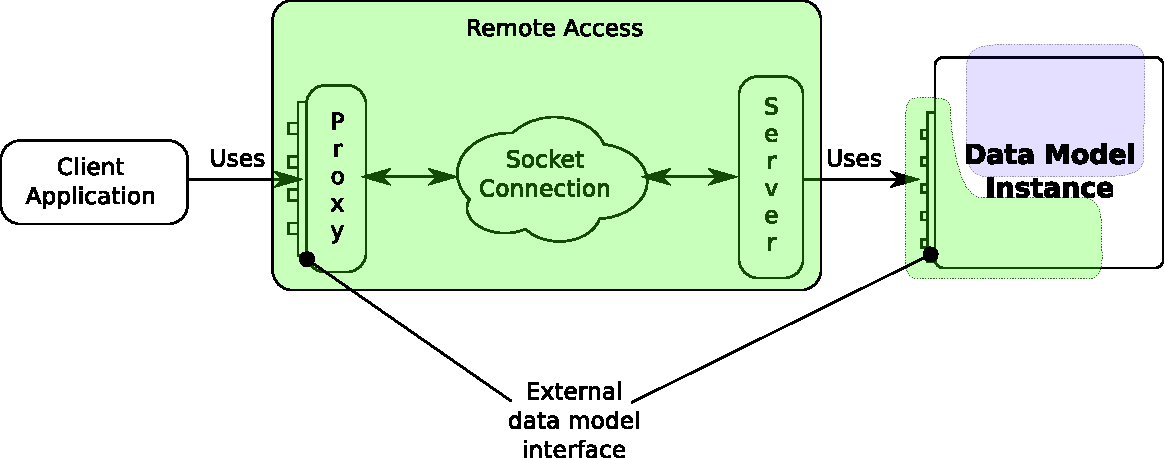
\includegraphics[scale=0.5]{img/remoteAccess.pdf}
\caption{A data model proxy interface and server is generated, to support transparent remote access to a data model instance. Coloured areas are auto generated code.}
\label{fig:remoteAccess}
\end{figure}


\subparagraph{Terminal test}

The generator also generates a program where a user can call the methods
of the external interface through a simple terminal.

\begin{figure}[h!]
\centering
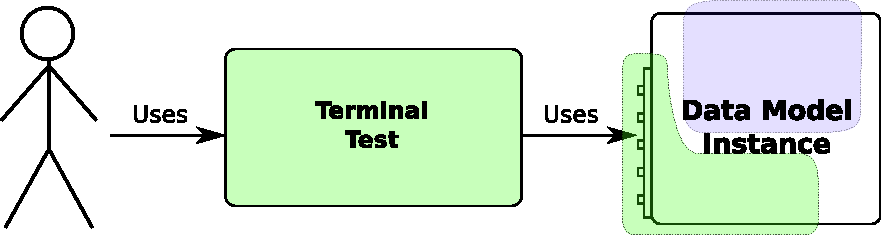
\includegraphics[scale=0.5]{img/terminalTest.pdf}
\caption{An terminal test program is generated to let a user test the methods in the external interface of a data model instance.}
\label{fig:terminalTest}
\end{figure}


\subparagraph{Web Interface}

It would also be possible to generate a web interface where a user
can interact with a data model instance through the external interface.
Javascript can be created to validate the value domains. We have created
an early prototype of this, but it requires a bit more work to be
perfected.

\begin{figure}[h!]
\centering
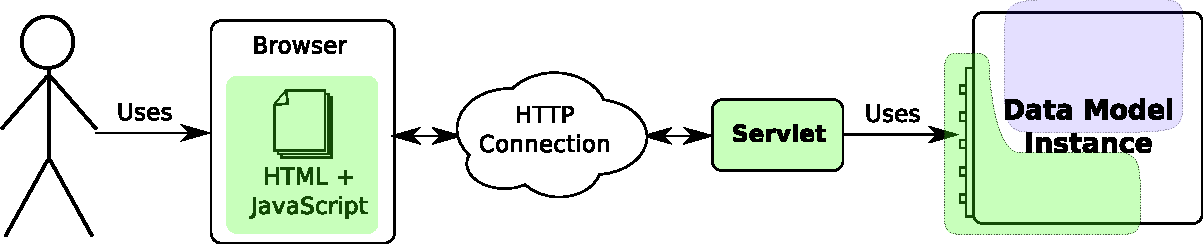
\includegraphics[scale=0.5]{img/web.pdf}
\caption{A web servlet for interacting with a data model instance together with HTML and Javascript for validating values on the client side, could be auto generated.}
\label{fig:web}
\end{figure}


\paragraph{Names and Packages}

It is important to us that the generated code can compile right away
without any changes, so we need to keep track of all imports and package
information. Since many of the generated interfaces and classes are
dependent on each other and on the runtime interface, any changes
to the naming conventions or the package structure would require lots
of changes to the generator code in many different places. To avoid
this we have abstracted out the naming conventions and the package
structure to a separate interface that takes care of all class names,
package names and package layout. This interface is then used all
over the generator. In this way it is easy to make changes to the
names of interfaces and classes or to the package structure of the
generated code. It is even possible to have several implementations
of the naming interface, so it is possible to switch between different
naming and package layout strategies.
